%% Author: Giacomo Minello

% The document class
% \documentclass{report}
% \documentclass{book}
\documentclass[12pt]{article}
 
\usepackage{graphicx}
\graphicspath{ {./figures/} }
\usepackage{wrapfig}
% babel english 
\usepackage[english]{babel}
%allow H on figures
\usepackage{float}

\usepackage{csquotes}

%indent chapters
\usepackage{indentfirst}


\setlength{\headheight}{14.5pt}

%allow subfigures
\usepackage{subcaption}

\usepackage{fancyhdr}
\pagestyle{fancy}
%references done right
\usepackage[
backend=biber,
sorting=none
]{biblatex}
\addbibresource{references/biblio.bib}

% cross-referenced element become links 
\usepackage[hidelinks]{hyperref}

%This will set the options to configure the behaviour of the links within the document. 
%Every parameter must be comma-separated and the syntax must be in the format parameter=value. 
\hypersetup{
    colorlinks=false,
    %linkcolor=black,
    %urlcolor=cyan,
    %pdftitle={PDF title},
    %pdfpagemode=FullScreen
}
\urlstyle{same}

\setlength{\parskip}{0.5em}
 

\title{The Stuxnet attack on the Natanz fuel enrichment plant in Iran\\
\large{Post attack analysis in a cyberwarfare scenario}
\rule[0.1cm]{13cm}{0.1mm}
\rule[0.5cm]{13.5cm}{0.6mm}}
\author{Group: Nuclear Pizza Toppings \\
Nicolò Diomedi, Gabriele Gallotti, Giacomo Minello
\\
\scriptsize‘‘[…] whoever provided the required intelligence may as well know the favorite pizza toppings \\
\scriptsize of the local head of engineering.’’\cite{killcentrifuge}
\\
}

% Set today date
\date{\today}
%set date to null to avoid showing it in maketitle
\date{}

\begin{document}
\begin{titlepage}
% create title
\maketitle
\begin{abstract}
\noindent  This document aims to provide an holistic view of the Stuxnet cyber attack on the Natanz fuel enrichment plant.
In the first part of this document we will provide a description of the plant and of the context in which it functioned. 
We will then illustrate the actual attack, the way in which it worked, and we will try to explain why it was so successful in its endeavour.
\end{abstract}
\end{titlepage}


% table of content 
\tableofcontents

\listoffigures

\newpage

\section{Introduction}
Natanz is an hardened Fuel Enrichment Plant (FEP) covering 100,000 square meters that is built 8 meters underground and protected by a concrete wall 2.5 meters thick, itself protected by another concrete wall. In 2004, the roof was hardened with reinforced concrete and covered with 22 meters of earth. The complex consists of two 25000 square meter halls and a number of administrative buildings. This once secret site was one of the two exposed by Alireza Jafarzadeh in August, 2002. IAEA Director General Mohamed ElBaradei visited the site on 21 February 2003 and reported that 160 centrifuges were complete and ready for operation, with 1000 more under construction at the site. Under the terms of Iran’s safeguards agreement, Iran was under no obligation to report the existence of the site while it was still under construction.

\begin{figure*}[ht!]
    \centering
    \begin{subfigure}[t]{0.5\textwidth}
        \centering
        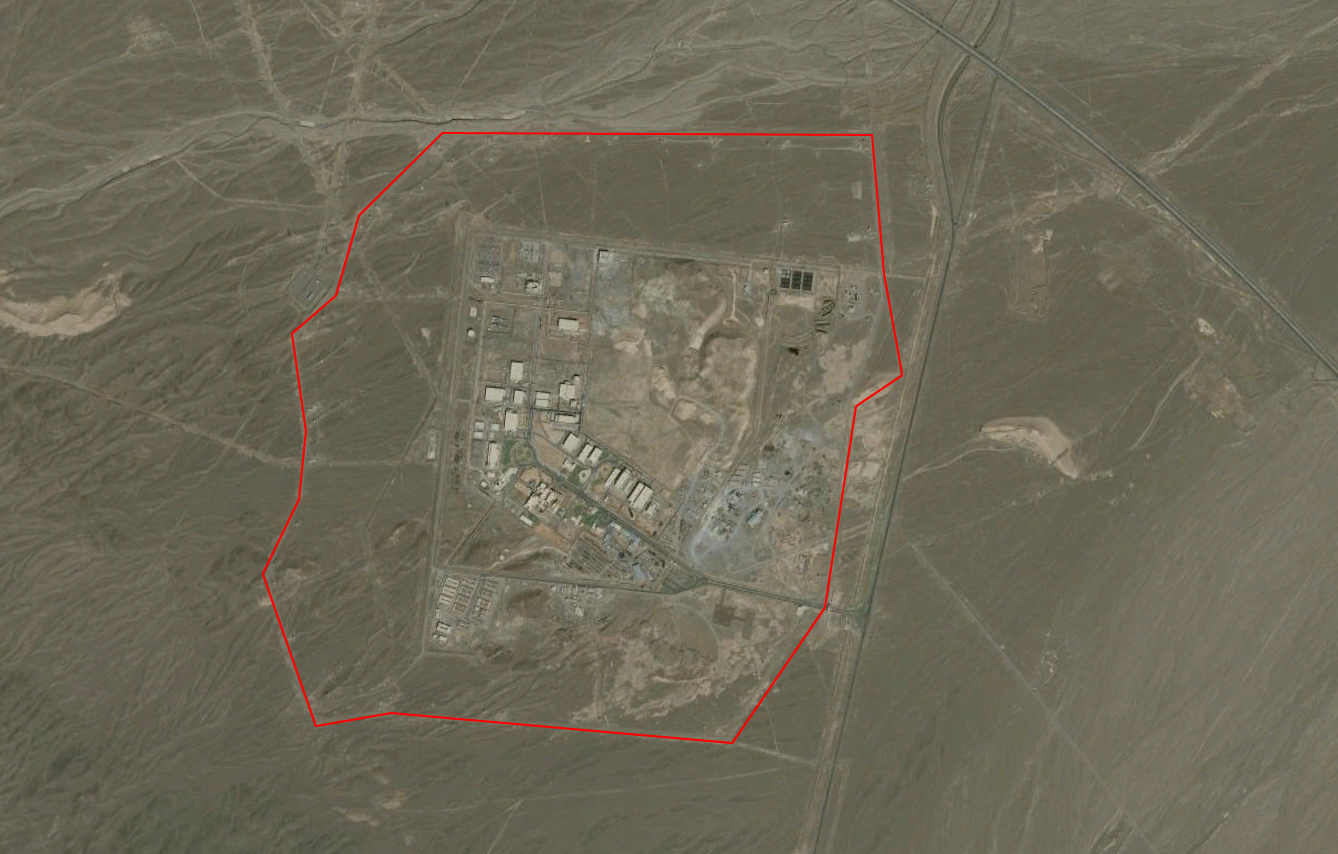
\includegraphics[height=0.65\textwidth]{natanz1.jpg}
        \caption{Highlighted: 4.7 miles security perimeter}
    \end{subfigure}%
    ~ 
    \begin{subfigure}[t]{0.5\textwidth}
        \centering
        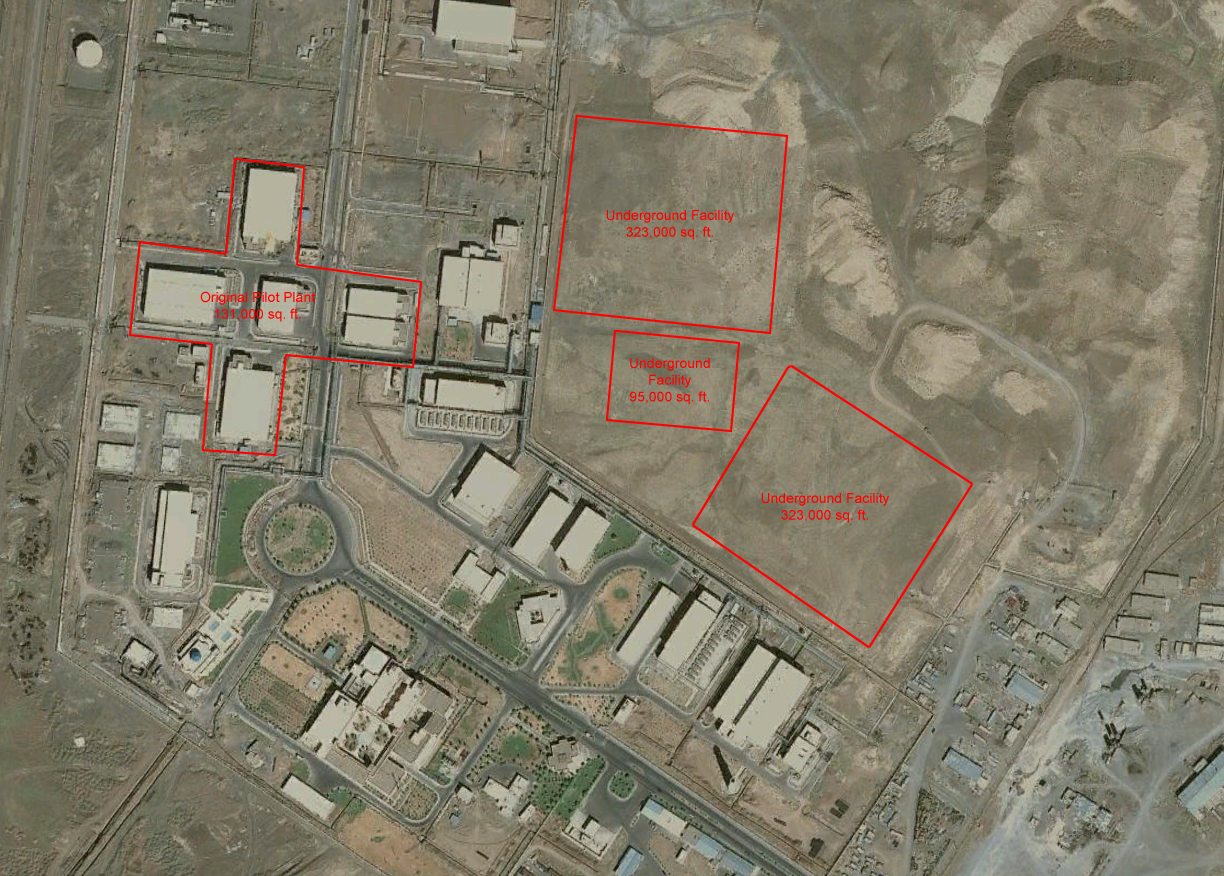
\includegraphics[height=0.65\textwidth]{natanz2.jpg}
        \caption{Buildings complex and underground structures}
    \end{subfigure}
    \caption{Natanz Fuel Enrichment Plant satellite images. \href{https://publicintelligence.net/iran-nuclear-site-natanz-uranium-enrichment-site/}{Source.}}
\end{figure*}

Iran's nuclear program was launched in the 1950s with the help of the United States as part of the Atoms for Peace program. Flush with oil money, the Shah of Iran publicly declared that he wanted to move forward with an ambitious nuclear energy program. For the Shah, as with Iranian leaders decades later, nuclear technology was not just a means of delivering security but also a matter of prestige, a means of restoring status to the proud Persian people who had once ruled an empire.  
In 1970, Iran ratified the Non-Proliferation Treaty (NPT), making its nuclear program subject to the IAEA's verification. The participation of the United States and Western European governments in Iran's nuclear program continued until the 1979 Iranian Revolution.

From 1984 nuclear research in Iran had begun to pick up under the Speaker of Parliament (and later President) Hashemi Rafsanjani. Rafsanjani was a wily, enigmatic politician who would become a key proponent of developing Iranian nuclear capability. His task would not be easy: the 1979 revolution had left Iran with a paltry scientific and technological base. Thousands of students were sent abroad again and Iran even tried to lure former scientists back to the country but this was largely unsuccessful.
In 1985 the Iranian leadership made the decision to begin work on its own enrichment program. Researchers were told to scour through publicly available technical literature for any clues on how to master the complex technology. But the Iranians would find that it was far easier to buy in outside help than do all the difficult research themselves. Slowly Iran began to master the complex technology. By 2000 Iran was ready to begin the construction of the two enrichment facilities at Natanz: the smaller pilot plant was to have one thousand centrifuges, the larger fifty thousand.

At the same time,  broad national consensus has also emerged domestically that backs Iran’s drive to acquire nuclear energy technology, partly because of reasons of national pride and self-perception as a regional power and partly because of the perceived security (not least against any U.S. plans for regime change) that having the capability to develop nuclear weapons might bring. That desire is heightened because Iran lives in a neighborhood where nearby states like Pakistan, India, Russia, and Israel are already nuclear. 

Since 2005, Iran's nuclear program has become the subject of contention with the international community, mainly the United States. Many countries have expressed concern that Iran's nuclear program could divert civilian nuclear technology into a weapons program. This has led the United Nations Security Council to impose sanctions against Iran which had further isolated Iran politically and economically from the rest of the global community. 

With negotiations over Iran’s nuclear program deadlocked, in 2006, the George W. Bush administration initiated a cyber-warfare operation, code-named “Olympic Games,” aimed at sabotaging Iran’s growing enrichment activities through a slow barrage of cyber-strikes.
The goal of the cyber attacks was not to destroy the nuclear program of Iran completely but to stall it enough for sanctions and diplomacy to take effect. This was successful as a nuclear treaty with Iran was reached in July 2015.


\section{Description of the system}
    \begin{wrapfigure}{L}{0.35\textwidth}
    \centering
    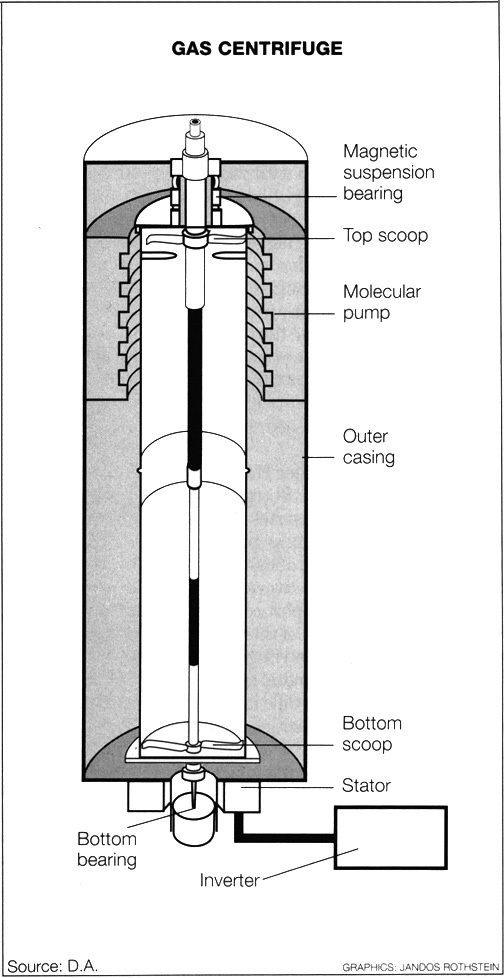
\includegraphics[height=0.65\textwidth]{figures/centrifugeAlternative.jpg}
    \caption{Centrifuge section}
    \label{fig:centrifuge1}
    \end{wrapfigure}
The backbone of Iran’s uranium enrichment effort is the IR-1 centrifuge which goes back to a European design of the late Sixties / early Seventies that was stolen by Pakistani nuclear trafficker A. Q. Khan. It is an obsolete design that Iran never managed to operate reliably. Reliability problems may well have started as early as 1987, when Iran began experimenting with a set of decommissioned P-1 centrifuges acquired from the Khan network. Problems with getting the centrifuge rotors to spin flawlessly will also likely have resulted in the poor
efficiency that can be observed when analyzing IAEA reports, suggesting that the IR-1 performs only half as well – best case – as it could theoretically. A likely reason for such poor performance is that Iran reduced the operating pressure of the centrifuges in order to lower rotor wall pressure. But less pressure means less throughput – and thus less efficiency.

Gas centrifuges used for uranium enrichment are assembled into groups to maximize efficiency. Centrifuges within one group, also called an enrichment stage, share the same feed, product, and tails piping.
The collective tails is then piped into the collective feed of the next stage on one side, as well as the collective product is piped into the collective feed on the other side.
A cascade unit at Natanz is made up of 18 cascades. According to public information, sub-units of six cascades share one feed station, one product station, and one tails station, as we can see in figure \ref{fig:cascade}.
    \begin{figure}[H]
    \centering
    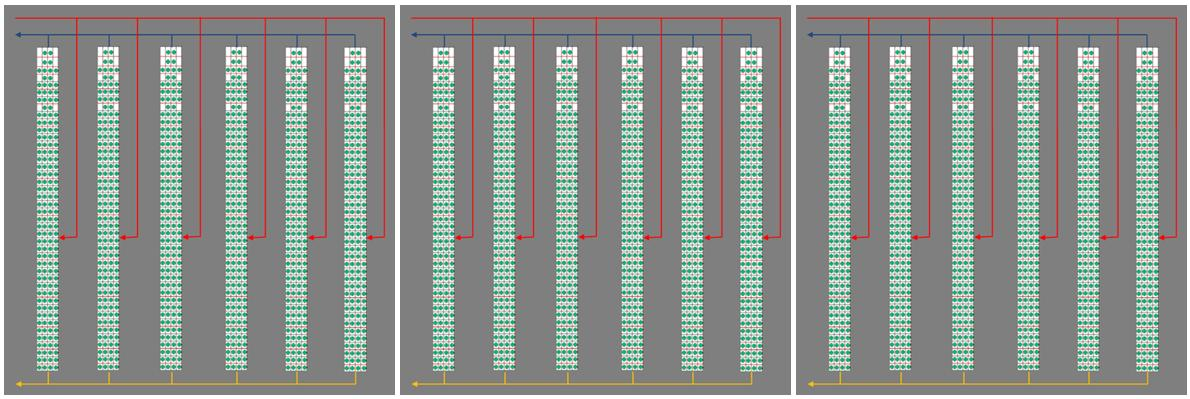
\includegraphics[height=0.33\textwidth]{cascade.png}
    \caption{Red piping indicates feed, blue piping indicates product, and yellow piping indicates tails.}
    \label{fig:cascade}
    \end{figure}
    
In order to use the thousands of fragile centrifuges without allowing the process to stop, Iran used a Cascade Protection System (CPS) which was designed to cope with ongoing centrifuge trouble by implementing a crude version of fault tolerance. The protection system was a critical component for Iran’s nuclear program as without it, Iran would not be capable of sustained uranium enrichment.

The CPS consisted of two layers, the lower layer being at the centrifuge level. Three fast-acting shut-off valves were installed for every centrifuge at the connectors of centrifuge piping and enrichment stage piping. By closing the valves, centrifuges that ran into trouble – indicated by vibration – could be isolated from the stage piping, said centrifuges were then run down and would then be replaced by maintenance engineers while the process kept running. The central monitoring screen of the CPS showed the status of each centrifuge within a cascade – running or isolated – as either a green or a grey dot.

 A dump system is present in any gas centrifuge cascade used for uranium enrichment but never used in production mode; it simply acts as a backup in case of cascade trips when the centrifuges must be evacuated and the “normal” procedure to simply use the tails take-off is unavailable for whatever reason. Iran discovered they can use the dump system to compensate stage overpressure. If that pressure exceeds a certain setpoint, the stage exhaust valve (controlled variable) is opened, and overpressure is released into the dump system until normal operating pressure is re-established.
this because when operating basically unreliable centrifuges, one will see shut-offs frequently, and maintenance may not have a chance to replace damaged centrifuges before the next one in the same enrichment stage gets isolated.


\section{Description of the cyber-event}

\subsection{SCADA}
SCADA in an acronym for Supervisory Control And Data Acquisition, a category of computer programs used to display and analyze process conditions. SCADA is only one component of an automated facility and does not directly interfere with actuator devices such as valves, pumps, or motors – this is achieved by industrial controllers that operate in real time and have no display and keyboard. SCADA can be considered the front-end of Natanz plant industrial process.

In particular a SCADA screen is usually organized to mimic the physical and/or functional layout of the plant, such as piping, and location of important system components. Engineers refer to that as a Piping and Instrumentation Diagram(P\&ID).
    
    \begin{figure}[H]
    \centering
    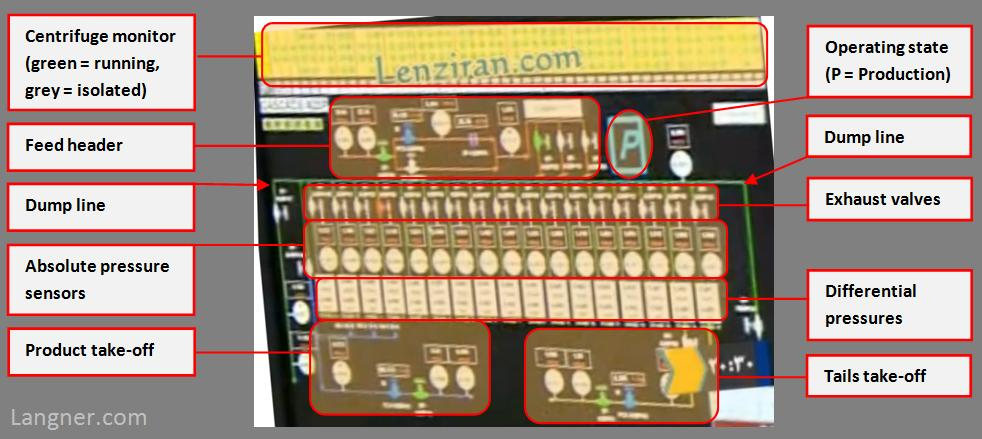
\includegraphics[height=0.45\textwidth]{scadaS.png}
    \caption{SCADA monitoring screen of the Cascade Protection System}
    \label{fig:scadaS}
    \end{figure}

The monitoring screen for the Cascade Protection System, shown in figure \ref{fig:scadaS}, shows the basic piping, valves, and pressure sensors of the cascades. Red piping (upper displayarea) signifies the feed header. Blue piping (lower left displayarea) signifies the product take-off, white piping (lower right display area) signifies the tails take-off, and green piping (upper display area, extending down left and right at the display borders) the pressure normalization and dump system.

Millibar readings in the rectangular black boxes (with “mbar” in red”) identify absolute pressure in the respective enrichment stage. The millibar readings in the white boxes stand for differential pressure and will most likely identify the delta between actual pressure and setpoint. An operator would observe the latter to spot potentially harmful trends, which could be identified by continuous high positive readouts. In contemporary Western SCADA software, one would most likely see such information displayed graphically. Centrifuge isolation valves are not shown, but their status can be determined in the centrifuge monitor area on top of the display. The centrifuge monitor area also allows to identify cascade shape easily. 

 \begin{figure}[H]
    \centering
    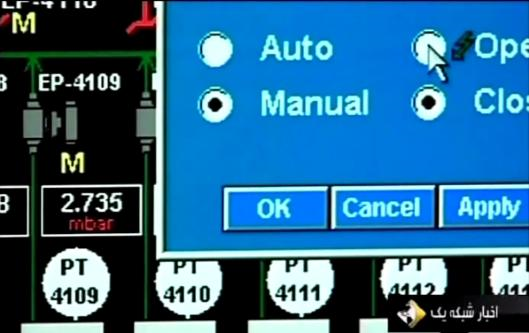
\includegraphics[height=0.6\textwidth]{scadaBlu.png}
    \caption{Millibar readings, particular of screen layout}
    \label{fig:scadaBlu}
    \end{figure}

Screen layout and functionality of the SCADA software appear quite amateurish by Western standards, and crude dialog boxes pop up every now and then on the CPS monitoring application. In modern SCADA software, such pop-up windows are rarely used because they obstruct other information on the display. Also, standard P\&ID symbols and labels have not been used consistently, suggesting that the application was custom-built by a corporation or individuals with little familiarity with contemporary SCADA software design.

\subsection{Stuxnet}
Stuxnet is the worm that targeted SCADA systems and the centrifuges of the Natanz plant causing substantial damage to the Iranian nuclear plan. It was also the first targeted weaponized cyber-attack against an industrial control system

Once installed on a PC, Stuxnet uses Siemens' default passwords to gain access to the systems that run the WinCC and PCS 7 programs which control and modify the code of the PLCs (programmable logic controller) which control the machines themselves Stuxnet operates in two stages after infection, according to Symantec Security Response Supervisor Liam O'Murchu. First it uploads configuration information about the Siemens system to a command-and-control server. Then the attackers are able to pick a target and actually reprogram the way it works. 

\subsection{Timeline of the attack}
    \begin{figure}[H]
    \centering
    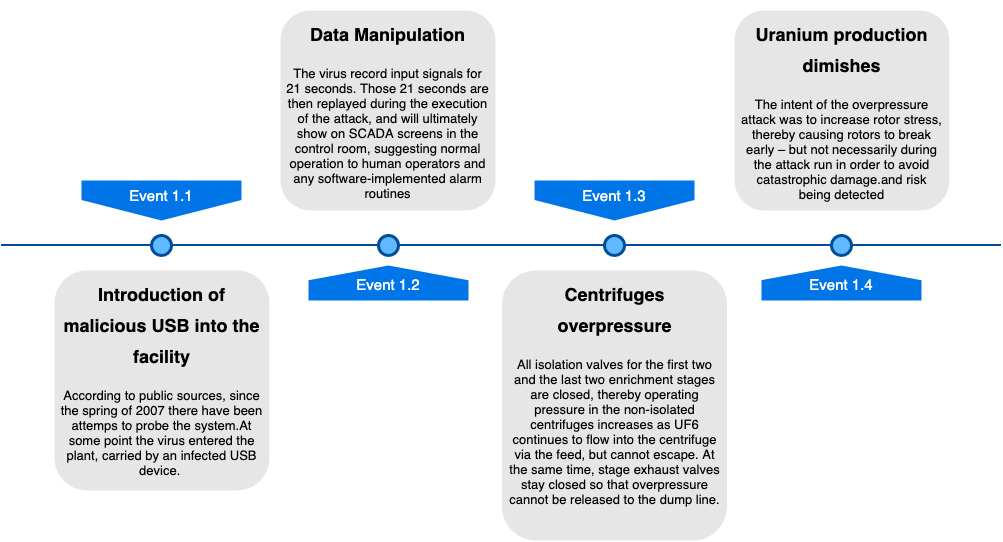
\includegraphics[height=0.5\textwidth]{time1.png}
    \caption{Timeline of the first phase of the attack}
    \label{fig:time1}
    \end{figure}
    
     \begin{figure}[H]
    \centering
    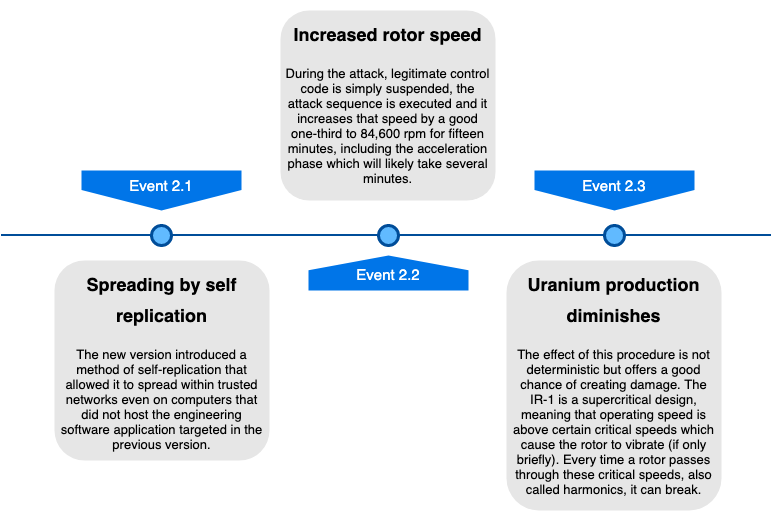
\includegraphics[height=0.6\textwidth]{time2.png}
    \caption{Timeline of the second phase of the attack}
    \label{fig:time2}
    \end{figure}

\section{Accident Analysis}
    \subsection{First phase}
    \subsubsection{Event 1.1 - Introduction of malicious USB into the facility}
    Since the spring of 2007 there have been multiple attempts to probe the system. At some point the virus entered the plant, probably carried by an infected USB device. According to four intelligence sources an Iranian engineer recruited by the Dutch intelligence agency AIVD provided critical data that helped the U.S. developers target their code to the systems at Natanz.
    
        \begin{figure}[H]
        \centering
        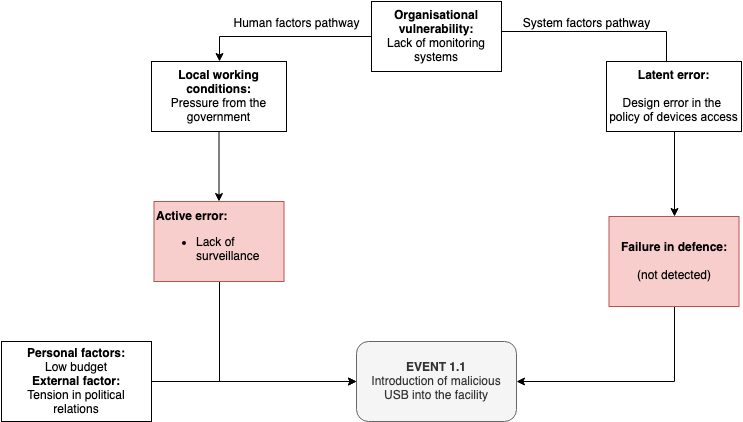
\includegraphics[height=0.6\textwidth]{event11.png}
        \caption{Event 1.1}
        \label{fig:event11}
        \end{figure}
        
    \subsubsection{Event 1.2 - Data Manipulation}
    The virus record input signals for 21 seconds. Those 21 seconds are then replayed during the execution of the attack, and will ultimately show on SCADA screens in the control room, suggesting normal operation to human operators and any software-implemented alarm routines
        \begin{figure}[H]
        \centering
        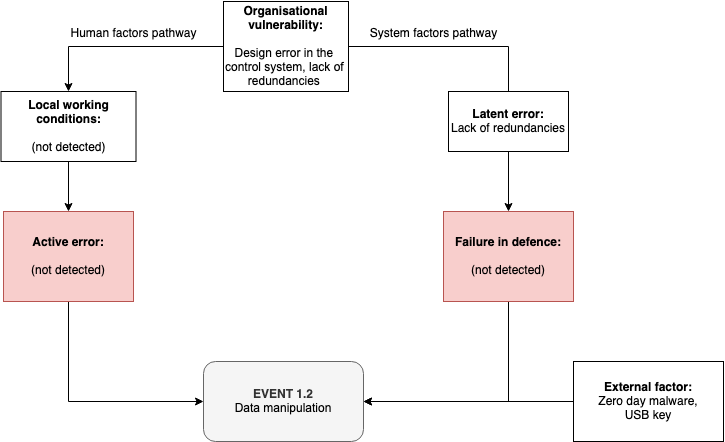
\includegraphics[height=0.6\textwidth]{event12.png}
        \caption{Event 1.2}
        \label{fig:event12}
        \end{figure}
        
    \subsubsection{Event 1.3 - CPS override}
    All isolation valves for the first two and the last two enrichment stages are closed, thereby operating pressure in the non-isolated centrifuges increases as UF6 continues to flow into the centrifuge via the feed, but cannot escape. At the same time, stage exhaust valves stay closed so that overpressure cannot be released to the dump line.
        \begin{figure}[H]
        \centering
        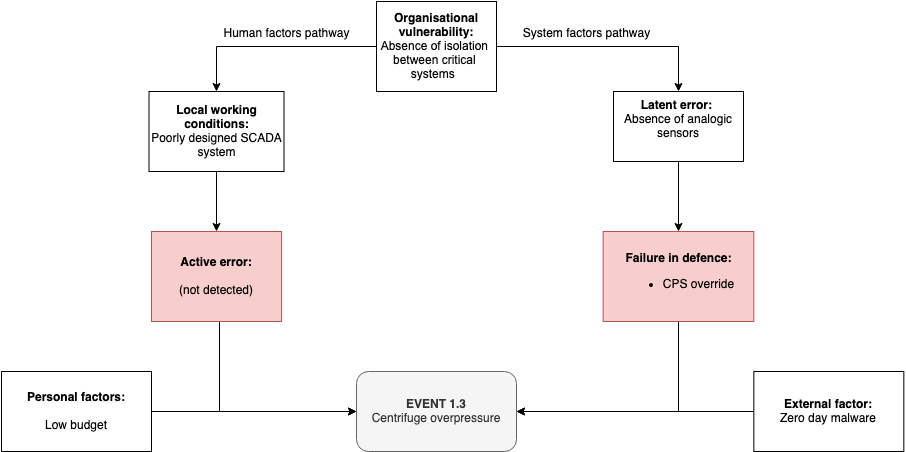
\includegraphics[height=0.6\textwidth]{event13.png}
        \caption{Event 1.3}
        \label{fig:event13}
        \end{figure}
        
      \subsubsection{Event 1.4 - Centrifuges failure}
      The intent of the overpressure attack was to increase rotor stress, thereby causing rotors to break early – but not necessarily during the attack run in order to avoid catastrophic damage.and risk being detected
        \begin{figure}[H]
        \centering
        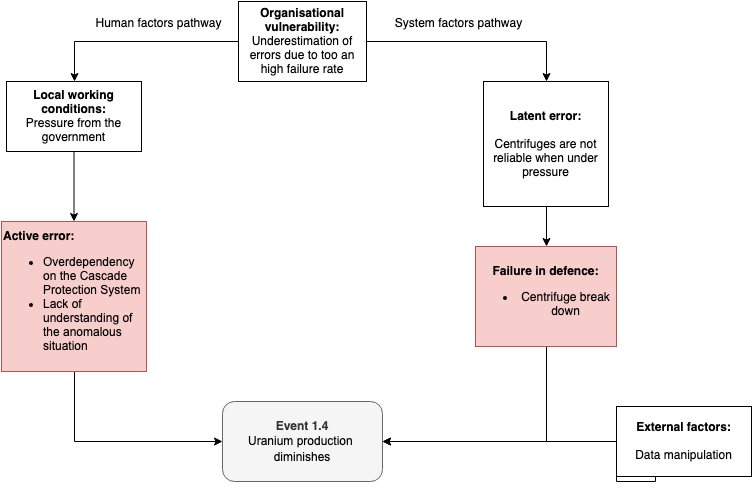
\includegraphics[height=0.6\textwidth]{event14.png}
        \caption{Event 1.4}
        \label{fig:event14}
        \end{figure}
        
    \subsection{Second phase}
    \subsubsection{Event 2.1 - Spreading by self replication}
    The new version introduced a method of self-replication that allowed it to spread within trusted networks even on computers that did not host the engineering software application targeted in the previous version.
    
        \begin{figure}[H]
        \centering
        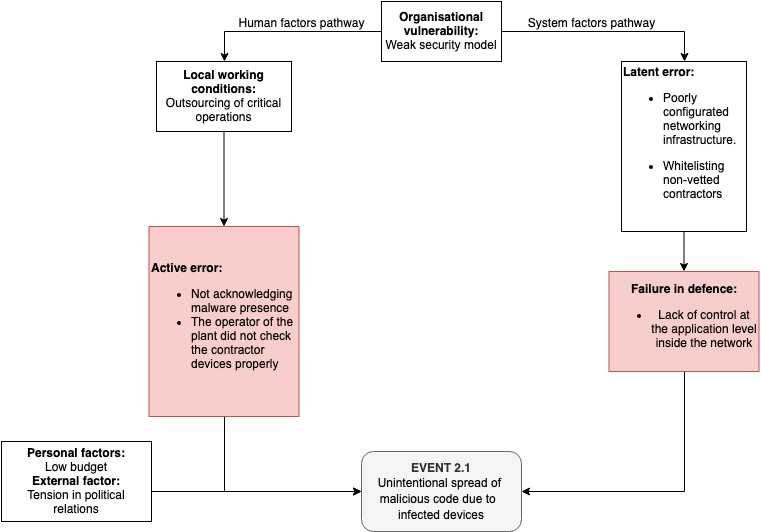
\includegraphics[height=0.6\textwidth]{event21.png}
        \caption{Event 2.1}
        \label{fig:event21}
        \end{figure}
        
    \subsubsection{Event 2.2 - Rotor attack}
    During the attack, legitimate control code is simply suspended, the attack sequence is executed and it increases that speed by a good one-third to 84,600 rpm for fifteen minutes, including the acceleration phase which will likely take several minutes.
    
        \begin{figure}[H]
        \centering
        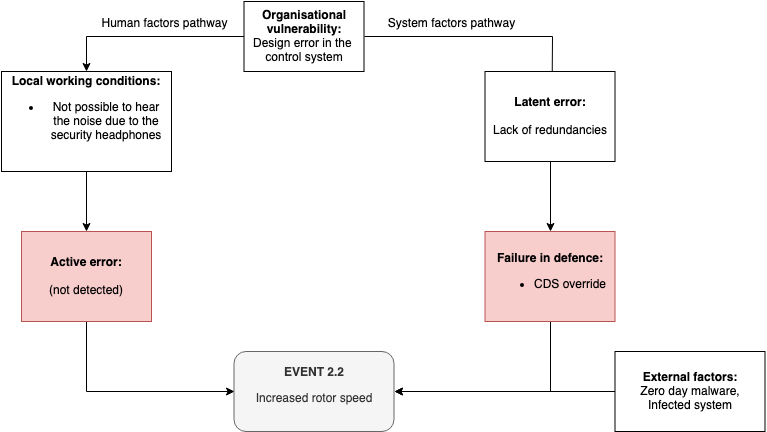
\includegraphics[height=0.6\textwidth]{event22.png}
        \caption{Event 2.2}
        \label{fig:event22}
        \end{figure}
        
    \subsubsection{Event 2.3 - Centrifuges failure}
    The effect of this procedure is not deterministic but offers a good chance of creating damage. The IR-1 is a supercritical design, meaning that operating speed is above certain critical speeds which cause the rotor to vibrate (if only briefly). Every time a rotor passes through these critical speeds, also called harmonics, it can break. 
    
        \begin{figure}[H]
        \centering
        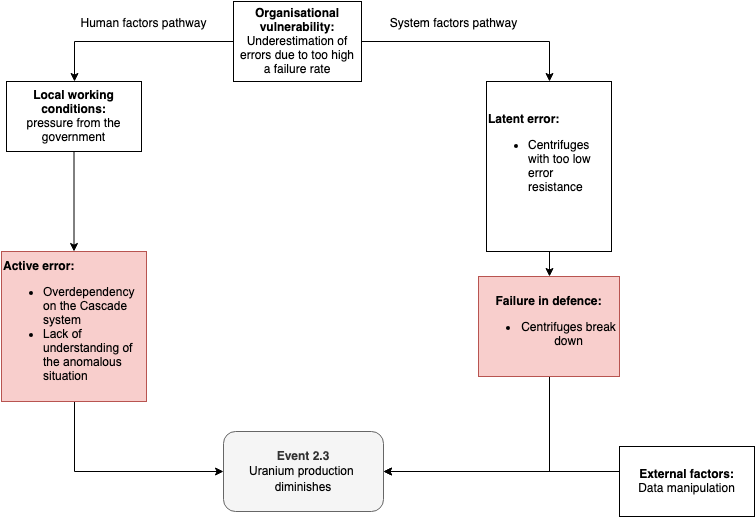
\includegraphics[height=0.6\textwidth]{event23.png}
        \caption{Event 2.3}
        \label{fig:event23}
        \end{figure}
        
\section{Conclusion}
The final considerations regarding stuxnet concern various aspects such as technological, social, political and economic ones.

From a internal political point of view, the fact  that Iranian authorities did not manage to protect their enrichment plant against a foreign cyberattack meant that they were discredited.
The malware had almost no direct effects on the Iranian population or society itself as it was designed to avoid collateral damage (Rosenbaum, 2012). Had the attack caused severe consequences and more powerful effects, including the potential loss of human lives, it might have led to an escalation of violence between Iran and the countries it believed to be responsible(Collins and McCombie, 2012, p. 88; Rosenbaum, 2012). 
Considering economic effects for Iran: being subject to international embargoes prevented access to international markets for buying nuclear-related materials and instead needed continue to make the centrifuges themselves.
Considering long-term economic repercussions caused by the cyberattack, the nation needed to manage delays in the production of low-enriched uranium. Moreover, establishing new security and cybersecurity measures in nuclear facilities to avoid the recurrence of an attack such as Stuxnet would have required a significant financial investment. 
The physical effect of Stuxnet was the damage caused to the centrifuges.
The physical consequences of Stuxnet were rather limited, but it was probably designed to remain hidden for a certain amount of time, damage the centrifuges and then disappear (Nakashima and Warrick, 2012).
From an international standpoint the attack showed that it is possible to build a highly sophisticated, offensive cybertool, and that perpetrators have the resources to accomplish such an attack. Moreover, this case demonstrates that separating a critical infrastructure network from the internet can no longer be considered an adequate security measure. States have realized that they need to take action in order to avoid falling victim to attacks of this nature. (cit)
We also have to consider that the worm leaked and spread to other computers outside Iran, this meant that anybody with the right competences would be able to reverse-engineer it, modify it to suit other purposes, sell it or use it (Collins and McCombie, 2012, p. 89).

The Stuxnet attack also impacted the definition of national cybersecurity policy.
States should particularly focus on computer users and the issue of using unknown USB drives.
The fact that the Natanz networks were separated from other networks did not sufficiently protect them against the malware. 
Even in Europe , which by 2006 had already created its security policy  in the form of the European programme on critical infrastructure protection (EPICIP), seemed to only cite briefly cybersecurity when discussing critical assets.
As a consequence, states started to integrate critical infrastructures in cybersecurity strategies.
For example in 2016 Europe defined the NIS directive, that made it mandatory to have a computer security incident response team (CSIRT) to which operators must report relevant incidents. 

The incident has shown that industrial equipment such as SCADA systems often suffers from weak cybersecurity standards. To diminish the risk of these vulnerabilities being exploited, states should have promoted technical standards indicating the level of cybersecurity of connected equipment at the international level.

The European Commission’s science and knowledge service is developing an IACS (Industrial and Automation Control Systems) cybersecurity components certification framework  that shall provide a mechanism to establish European cyber-security certification schemes. The IACS framework will also attest that the ICT products, ICT services and ICT processes that have been evaluated in accordance with such schemes comply with specified security requirements for the purpose of protecting the availability, authenticity, integrity or confidentiality of stored, transmitted or processed data throughout their life cycle. The general structure of  the certifications range between a self declaration of compliance (ICCF) to a certification of full cyber resilience (ICCS-A) designed for highly critical markets. So vendors will need to demonstrate that they have eliminated involuntary and malevolent opportunities to introduce vulnerabilities.


\begin{flushright}
Nicolò Diomedi
\end{flushright}
\\~\\
\begin{flushright}
Gabriele Gallotti
\end{flushright}
\\~\\
\begin{flushright}
Giacomo Minello\\

\includegraphics[scale=0.06]{figures/firmaMinello.png}
\end{flushright}

% print biblio with heading in the index
\newpage
\printbibliography[heading=bibintoc]
\end{document}
